\documentclass{article}
\usepackage{amsmath}
\usepackage{graphicx}
\usepackage{xcolor}
\usepackage{geometry}
\usepackage{hyperref}
\usepackage[linewidth=1pt]{mdframed}
\geometry{a4paper,left=20mm,right=20mm,top=20mm,bottom=20mm}
\hypersetup{colorlinks=true,linkcolor=blue,filecolor=blue,citecolor = black,urlcolor=blue}
\usepackage{matlab-prettifier}

\makeatletter
\newcommand{\xRightarrow}[2][]{\ext@arrow 0359\Rightarrowfill@{#1}{#2}}
\makeatother

\title{Growth curves analysis}
\author{Marco Mauri}

\begin{document}

\maketitle

\section{Modelling microbial growth}
A small internal note on how the curve-fitting software in MATLAB operates. The aim of this document is both to provide insight in the functionality of the software and justify the statistical approach used to analyse the growth curves coming from the plate readers (OD vs time). The process is intended to extract some biological parameters by using phenomenological models of growth, detailed in the following. It includes extension to any physiological model, including dynamical model via ODEs, if the model has a closed form with unknown parameters.

\subsection{Quick usage}
The user needs to run section by section the script. The first part analyses separately the experiments that need to be averaged (technical or biological replicates averaged over the same conditions). To do that, the excel files and the position on the plate are declared in an external text (.m) file. The excel file where to retrieve the background information, the excel file for the experiments, and the respective well positions are provided as follow 
\begin{lstlisting}[frame=single,numbers=left,style=Matlab-Pyglike]
inputs.expN = 1; %a number for your reference, different for each analysis
inputs.fileDataBkg = 'bkgfile'; %bkg file(s)
inputs.bkgWells = {[13,18,25,30]}; %bkg wells
inputs.fileDataExp = 'expfile'; %exp file(s)
inputs.expWells = {[14:17,26:29]}; %exp wells
inputs.tinFit = {[]}; %initial time for fit
inputs.tfinFit = {[169]}; %final time for fit
inputs.modelN = 11; %number of model for fitting

inputs.tin = {[]}; %initial time for the exp
inputs.tfin = {[]}; %final time for the exp
inputs.averagecurves = 1; %0 no, 1 yes
inputs.reanalysis = 1; %0 do only fit, 1 analysis + fit
inputs.fitYN = 1; %fit 1 yes 0 no
\end{lstlisting}
It is also possible to analyse or fit just a part of the experiment by restricting the time window. This file is read and a creates a structure with the information provided to the script.
\begin{lstlisting}[frame=single,numbers=left,style=Matlab-Pyglike]
%% add script and data folders
addpath(genpath('script'));

%% analysis for each data file
inputs = struct();
inputs.folderData = 'dataRebecca'; %folder

file_inpunt = 'a1'; %parameter file just created
run(strcat(inputs.folderData,'/',file_inpunt,'.m'))
analysisFit(inputs)
\end{lstlisting}
The user has to create a file for each condition to average. The analysis save in separate folders with the experiment name the output and several MATLAB files and excel files are created. Then, several conditions can be load and plotted. This is done by creating a second text file (.m) as
\begin{lstlisting}[frame=single,numbers=left,style=Matlab-Pyglike]
parameterAnalisis.name_condition = 'xylMIN65'; %name the condition
parameterAnalisis.exps_to_load = [21,22,23]; %exps to load, same name as they where saved
parameterAnalisis.convert_unit = 2; %0 sec, 1 min, 2 h choose the time unit
parameterAnalisis.condition_media1 = 6.5; %a firts tag 
parameterAnalisis.condition_media2 = 'xylMIN'; %a second tag

parameterAnalisis.condition_ylabel = 'Growth rate'; %what to plot
parameterAnalisis.parameter_to_plot = 4; %where to retrieve the data to plot
parameterAnalisis.condition_names = {'0','1.5','30'}; %label of the plot
parameterAnalisis.condition_value = [0,1.5,30]; %values of the label
\end{lstlisting}
and running
\begin{lstlisting}[frame=single,numbers=left,style=Matlab-Pyglike]
%% load and plot several datasets + analysis parameters
parameterAnalisis = struct();
parameterAnalisis.inputs_folderData = 'dataAriane'; %folder
parameterAnalisis.name_condition = 'xylMIN65'; %parameter file

run(strcat(parameterAnalisis.inputs_folderData,'/',parameterAnalisis.name_condition,'.m'))
analysisParameters(parameterAnalisis)
\end{lstlisting}
Some plot regarding the query (here growth rate) are generated along with the excel files and .m files. The file AnalysisFit.m contains all the model to fit and the vector to store arranged as 
\begin{lstlisting}[frame=single,numbers=left,style=Matlab-Pyglike]
[1 klag,2 tlag*,3 q,4 mu,5 tswitch*,6 kswitch,7 ks--,8 t--,9 k--,10 tdeath*,11 kdeath,12 m, 13 x0*, 14 k*, 15 k2*, 16 k3*]
\end{lstlisting}
where each entry is a model parameter. For example, the growth rate is in the entry 4.

\subsection{Details of the script}
In the following sections, we detail some of the main functions of the script.

\subsection{Adding the paths}
The mains are saved in the upper folder and all the functions are stored in the subfolder \textit{script}. Data are stored in a separate folder with a custom name, e.g. \textit{data}. The first section of the main, e.g. $mainEx.m$, adds these paths to the MATLAB paths.
\begin{lstlisting}[frame=single,numbers=left,style=Matlab-Pyglike]
addpath(genpath('script'));
addpath(genpath('data'))
\end{lstlisting}

\subsection{Organisation of the microplate}
The wells in the microplate are numbered following rows and then columns in increasing order: A1=1, A2=2,...,A12=12, B1=13,...,B12=24, H12=96. This is the order that will be used in the software to identify the wells.

\begin{center}
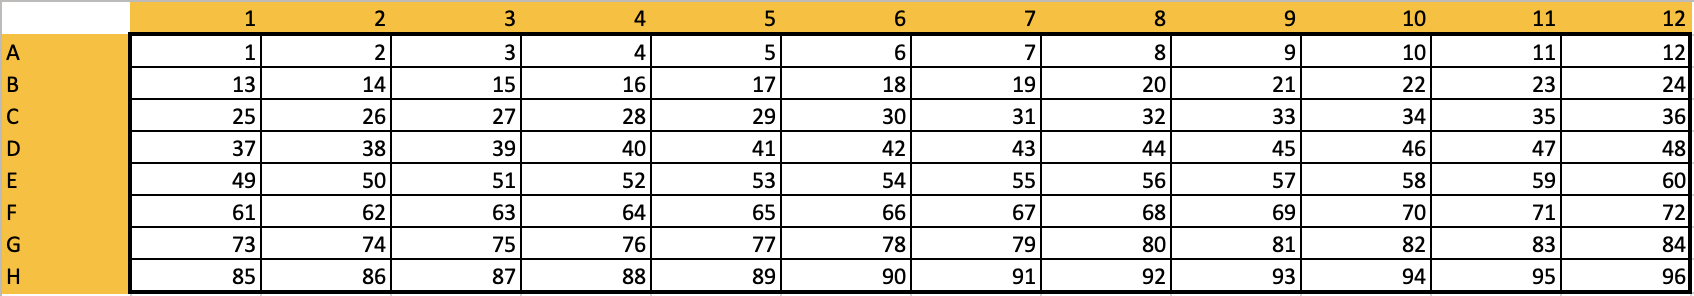
\includegraphics[width=0.6\textwidth]{plate} 
\end{center}

\subsection{Organisation of the Excel file}
The Excel file must contain in the first column the time in seconds, in the following columns the OD reading. All the wells must be listed in the file. If some wells are empty, just leave the column empty.

\subsection{Background analysis}
To properly subtract the background from the OD, we import the background from the excel file. The same biological replica can be stored in several files, any of each corresponding to a background in different wells. The time for the reading can be also an interval and it is not needed to have the same length. The script looks for the shortest time for the fitting. The background can be either computed and saved, or load if already previously stored. The user can choose to work in seconds, minutes, or hours.
\begin{lstlisting}[frame=single,numbers=left,style=Matlab-Pyglike]
bkg = struct(); %create a structure to store the results
bkg.filenames = {'data/file1.xlsx','data/file2.xlsx'}; %excel files
bkg.wells = {[13,18,19],[1,42,17]}; %wells in file1 and file2

%for more files subfields are created such as bkg.var{number}

bkg.tin = {[],[]}; %initial time, [] for initial time {[];[]};
bkg.tfin = {[6:46],[8:50]}; %final time, [] for maximal possible final time {[];[]};

% create or load the background
bkg.bkgAnalysis=1; %0 load, 1 create
bkg.minut=1; %1 minutes, 0 seconds, 2 hours
\end{lstlisting}
The script then fit the background to a model with initial guess for the parameters. Leave k0 empty for a polynomial model, positive for a saturating model, negative for a repression model.
\begin{lstlisting}[frame=single,numbers=left,style=Matlab-Pyglike]
if bkg.bkgAnalysis==1

    bkg.a0 = 1e-8;%1e-8;
    bkg.n = 1.3;
    bkg.k0 = []; %for polynomial model, negative for repression model

    [bkg1] = find_bkg(bkg);
\end{lstlisting}
If you need to store and save several backgrounds, remember to change the saved name or the folder where you store it to avoid rewriting it. The models for the OD background vs time are
\begin{enumerate}
\item Polynomial 
\begin{align}
f = a \cdot t^n + b
\end{align}
\item Saturation 
\begin{align}
f = a \frac{t}{t+k0} +b
\end{align}
\item Repression 
\begin{align}
f = a \frac{k0}{t+k0} +b
\end{align}
\end{enumerate}
The script before fitting finds the mean and standard error (from now on std) of the background
\begin{lstlisting}[frame=single,numbers=left,style=Matlab-Pyglike]
[bkg.mean,bkg.std] = MeanAndPlot(bkg.time{1},bkgR);
\end{lstlisting}
The fit is performed by minimising the weighted chi-square function
\begin{align}
\chi^2 = \sum \frac{(X_o - X_e)^2}{\sigma^2}
\end{align}
where $X_o$ and $X_e$ are the observed OD and predicted by the model OD, respectively, and $\sigma$ the std of the data if available. The script find the best parameters that minimise such function
\begin{lstlisting}[frame=single,numbers=left,style=Matlab-Pyglike]
modelChi = @(P) minimizeChiSquareBkg1(P,blackboxmodel,bkg.time{1},parameters0,Data0);
%minimize chi square
[fittedParameters,fval] = fminsearchbnd(modelChi,P00,lb,ub,options);
\end{lstlisting}
then it computes also the std of the fitted parameters and the confidence intervals at 95\% (CI) for the data (described in the following), and finally it plots the results. In black the average and std of the raw data and in red the best fit and the CI.
\begin{center}
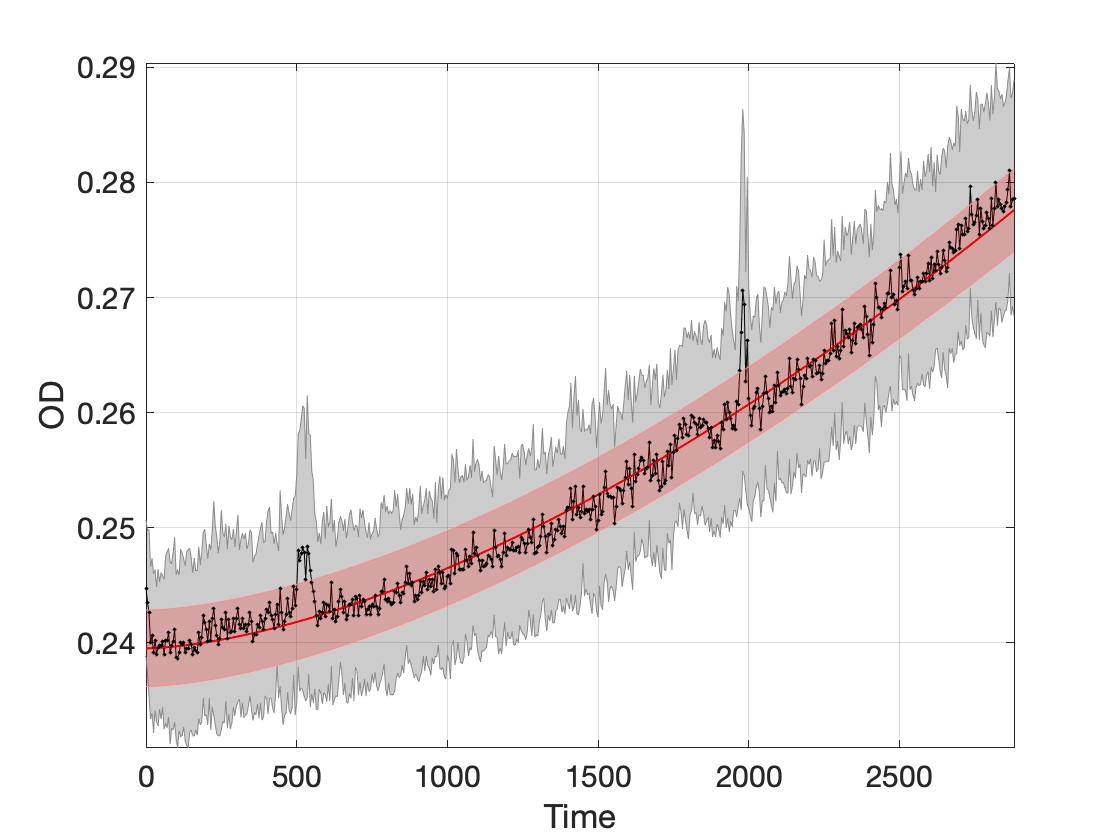
\includegraphics[width=0.6\textwidth]{b1} 
\end{center}
Now we have the background function that can extended at any time point and can be subtracted from the experimental data at any time position. The solution for the best fit are stored in the structure bkg along with the standard errors.

\subsection{Experimental data and background subtraction}
Similarly to the background, we define the files where to obtain the experimental data. We might have several biological replicates and for more than one technical replicate. They are necessary not only to reduce the experimental errors but also to identify stochastic processes. If the same technical replicates show a tested variation, the process might be stochastic. Such a statistical test is not included in this code. For a single biological replica use
\begin{lstlisting}[frame=single,numbers=left,style=Matlab-Pyglike]
experiment.filenames = {'data/exp1.xlsx'};
experiment.wells = {[14:17,26:29]}; %wells where exp is stored

experiment.tin = {[]}; %initial time, [] for initial time
experiment.tfin = {[]}; %final time, [] for maximal possible final time

experiment.smoothstrength = []; %you might want to smooth noisy data, use a positive number 

%bkg subtraction and average
[Data1,experiment1] = ExperimentSubtractBkg(experiment,bkg1);
save('data/Data1.mat','Data1') 
save('data/experiment1.mat','experiment1')
\end{lstlisting}
For more biological replicas change Data1 into Data2 etc and same for experiment1. Store and save them every time and then after such analysis for each biological replica, import them into a structure. The script plot all the data: raw data, averaged over technical replicate, and background subtracted data so that the user can verify possible stochastic events. The script in the function ExperimentSubtractBkg finds the mean and std of the technical replicates
\begin{lstlisting}[frame=single,numbers=left,style=Matlab-Pyglike]
[experiment.rawmean,experiment.rawstd] = MeanAndPlot(experiment.time{1},expR);
experiment.mean = experiment.rawmean-bkg.fit; %subtract mean
experiment.std = sqrt((experiment.rawstd).^2 + (bkg.fitStd).^2); %find std
\end{lstlisting}
The background subtraction is performed following a statistical approach and error propagation where the new variance is given by
\begin{align}
\sigma^2 = \sigma_{exp}^2 + \sigma_{bkg}^2 
\end{align}
In the Figure the raw data of the technical replicates, the average and std in black, the background in red, and the bkg-subtracted data in green. 
\begin{center}
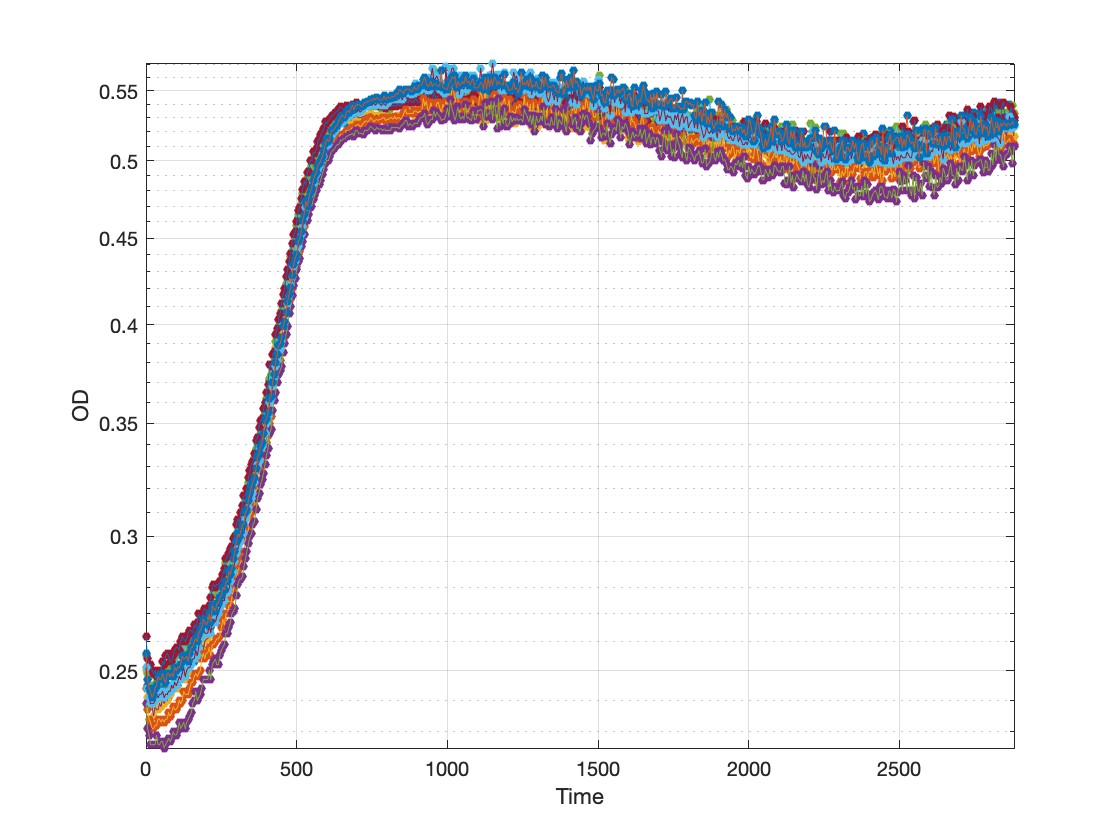
\includegraphics[width=0.45\textwidth]{e1} 
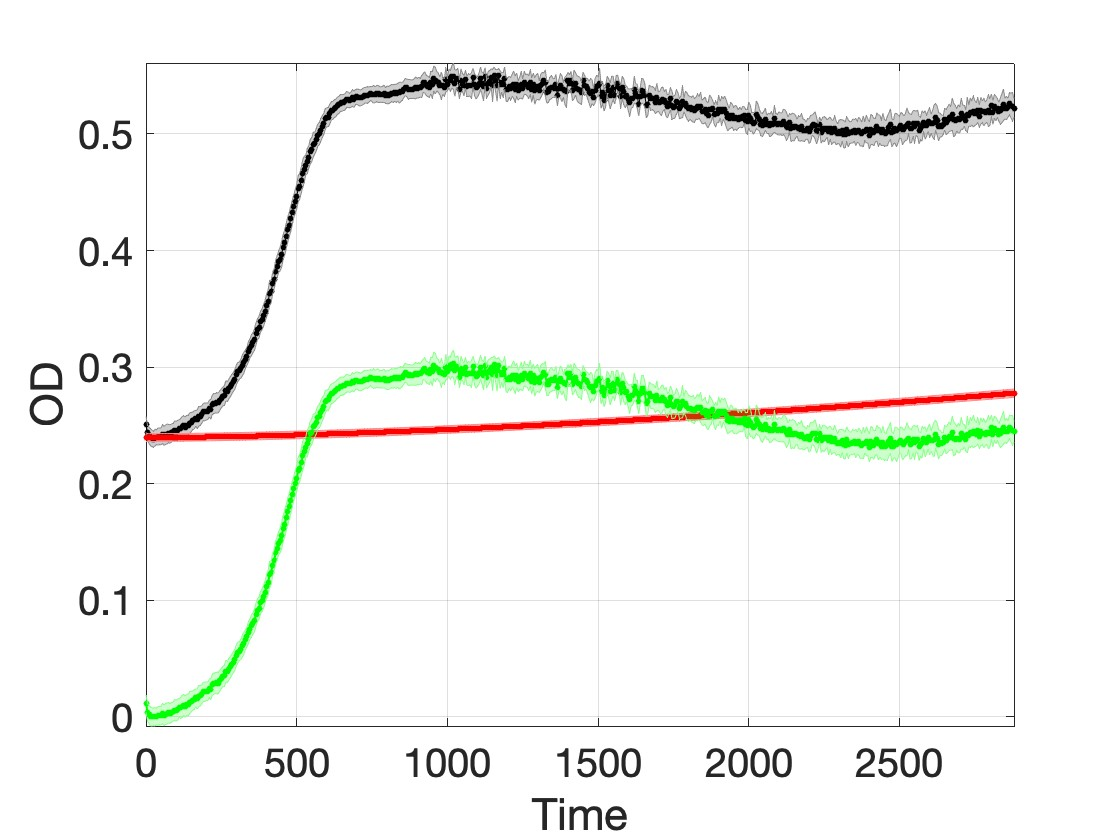
\includegraphics[width=0.45\textwidth]{e2} 
\end{center}
Then, if more biological replicate are available, the script analyse them and if the user want to average them, the script perform the instruction. The std error is computed again following error propagation. The user needs to load and store the different biological replicates in a structure
\begin{lstlisting}[frame=single,numbers=left,style=Matlab-Pyglike]
DataReplica.t{1} = Data1.time;
DataReplica.t{2} = Data2.time;

DataReplica.r{1} = Data1.XmeanSmooth;
DataReplica.r{2} = Data2.XmeanSmooth;

DataReplica.s{1} = Data1.Xstd;
DataReplica.s{2} = Data2.Xstd;

%average over replicas
Data = averageNsets(DataReplica);
\end{lstlisting}

Data about time, mean and standard deviation are saved in the structure Data.time, Data.Xmean and Data.Xmean, Data.Xstd, respectively. If the parameter $nomean$ is to 1, only the background subtraction is performed. If the parameter $bkg_subract$ is set to 0, no background subtraction is performed. If a file name is provided, the analysis is saved in an external excel file.

\subsection{Phenomenological models to extract the physiological parameters}
The script accept different types of models. The model can be passed both as system of ODE and as functions. To analyse the growth curves, we use piecewise functions. The final model consist in patching together several block functions. In the following, we present some of this block functions to extract the parameters. In any case, the drug and the nutrients concentrations are supposed to stay constant. To create piecewise function that start at $t_0$, we use Heaviside delta function $\theta(t-t_0)$. If we indicate with $X$ the OD, remember that the final point of a function is the $X_0$ of the new one and that the function in the new section must have time translated properly, e.g. $\exp (\mu (t-t_0))$ instead of $\exp (\mu t)$.

\subsubsection{Exponential growth}
\begin{align}
\frac{dX}{dt} &= \mu X \\
x(t) &= X_0 e^{\mu t}
\end{align}

\subsubsection{Exponential growth with saturation - logistic}
\begin{align}
\frac{dX}{dt} &= \mu X \left( 1 - \frac{X}{K} \right) \\
x(t) &= \frac{ X_0 e^{\mu t}}{1 + \frac{X_0}{K} (e^{\mu t}-1)}
\end{align}

\subsubsection{Lag exponential growth - Baranyi model}
\begin{align}
\frac{dX}{dt} &= \mu \frac{q(t)}{1+q(t)} X \\
\frac{dq}{dt} &= \mu q\\
x(t) &= X_0 \frac{1+q_0 e^{\mu t}}{1+q_0}
\end{align}

\subsubsection{Lag exponential-saturation growth}
\begin{align}
\frac{dX}{dt} &= \mu \frac{q(t)}{1+q(t)} X \left( 1 - \frac{X}{K} \right)\\
\frac{dq}{dt} &= \mu q\\
x(t) &= X_0 \frac{1+q_0 e^{\mu t}}{1+q_0 -q_0 \frac{X_0}{K} + \frac{q_0 X_0}{k} e^{\mu t}}
\end{align}

\begin{center}
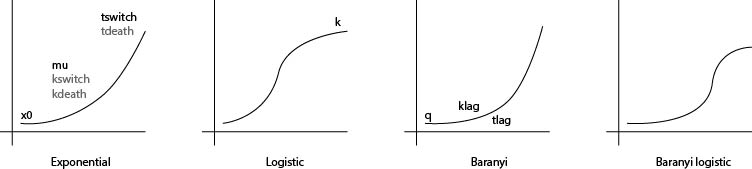
\includegraphics[width=0.9\textwidth]{models}
\end{center}

\subsection{Fit data to the model}
To fit the data to the model, we define a vector of initial guesses for the parameters, we decide whether to use the weighted chi-square, whether to use either a statistics methods or a bootstrapping methods to find the std of the best estimated parameters, and to find the CI either for the function or the new data. Then we decide which specific model to use.
\begin{lstlisting}[frame=single,numbers=left,style=Matlab-Pyglike]
parameters0 = [NaN,NaN,1e-5,0.012,243,-2e-4,NaN,NaN,NaN,468,-7e-5,1,NaN,NaN,NaN,NaN]; %initial guess

parametersFit = struct();
parametersFit.Chistd=1; %use std as weight in fit
parametersFit.nbootstrap = []; %[] empty for no bootstrap, number for n of bootstraps %boostrap to find error on fit parameters
parametersFit.confidenceprediction = 0; %0 95% confidence interval of fit function, 1 95% of finding new data in the interval

m = parameters0(12); %number of the ready-made model
if m==1
    [Data,parametersFit] = fitESED(Data,experiment.tin{1},experiment.tfin{1},parameters0,expN,parametersFit); %exp+saturation - exp - exp death
    ...
end
\end{lstlisting}
For example here we have initial guess related to these parameters
\begin{lstlisting}[frame=single,numbers=left,style=Matlab-Pyglike]
parameters0 = [1 klag,2 tlag*,3 q0,4 mu0,5 tswitch*,6 kswitch,7 ks--,8 t--,9 k--,10 tdeath*,11 kdeath,12 m ,13 x0*, 14 k*, 15 k2*, 16 k3*];
\end{lstlisting}
Remember that time is given in plate reader cycles. Star means that those parameters can be left as NaN, we use NaN as empty values.Then we perform the action to fit the data. The script looks for the best initial guess of the parameters that were not provided with an initial guess, such as time points for switching from one model to the others, or carrying capacities. Next, a model is defined
\begin{lstlisting}[frame=single,numbers=left,style=Matlab-Pyglike]
%define the model
blackboxmodel = choosemodel(m);

if m==1
    blackboxmodel = @ModelSaturationSwitchDeath;
    ...
end
\end{lstlisting}
The best fit is found by passing upper and lower limits for the parameters, this speed up the computation. The chi-square is minimized and the best fit is given as result.
\begin{lstlisting}[frame=single,numbers=left,style=Matlab-Pyglike]
%model chi square
modelChi = choosechisquare(m,blackboxmodel,time,param,Data);

%minimize chi square
[fittedparameters,~] = fminsearchbnd(modelChi,P0,lb,ub,options);
\end{lstlisting}
fittedparameters contains the best estimate for the fitted parameters.

\subsubsection{Standard error on the fitted parameters}
Now, we have to compute the standard error on the fit. This is done by following a statistical procedure. The inverse of the Hessian matrix of the chi-square with respect to the parameters to fit is the covariance matrix, which diagonal elements are the variance for each parameter. 
\begin{align}
U_{\alpha, \beta} &= \frac{1}{2} \frac{\partial ^2 \chi ^2 }{\partial \alpha \partial \beta}\\
Cov(\alpha,\beta) &= (U^{-1})_{\alpha, \beta}
\end{align}
where $\alpha$ and $\beta$ are two of the parameters to estimate. Therefore
\begin{lstlisting}[frame=single,numbers=left,style=Matlab-Pyglike]
%compute std of fitted parameters
f = modelChi; %define the chi-square model
P0 = fittedparameters; %define the varying parameters
H = chessian(f,P0); %compute the hessian
U = H./2; 
S = abs(inv(U)); %find the inverse of H/2
fittedparametersStd = zeros(size(fittedparameters,1),size(fittedparameters,2)); %extract the variance on diagonal
for l=1:size(fittedparameters,2)
      fittedparametersStd(l) = sqrt(S(l,l));
end
\end{lstlisting}
and the best parameter and the errors are stored
\begin{lstlisting}[frame=single,numbers=left,style=Matlab-Pyglike]
%best parameters
param.mu = fittedparameters(1);

%best fit
Xfit = blackboxmodel(time,param);
Data.Xfit= Xfit;
\end{lstlisting}
The script offers a second way to obtain such errors, the bootstrapping method. This doesn't suffer of approximation, since the method before is only valid for independent, normal distributed, and with small error parameters. For non-linear model a bootstrapping method is more accurate. Thus, $nbootstrap$ new datasets are bootstrapped by sampling the residual and adding them to the best fit. The resulting datasets are fitted, for each parameter $nbootstrap$ value are obtained and the mean and the std computed. 
\begin{lstlisting}[frame=single,numbers=left,style=Matlab-Pyglike]
%mean, std and ci of paramters (not data!) via bootstrapping
resid = Xfit-X;
bs = bootstrp(parameters.nbootstrap,@(bootr)bootF(param,Data,bootr,blackboxmodel,time,P0,lb,ub,options,m),resid);
se = std(bs); %std error of fitted parameters
for l=1:size(fittedparameters,2)
    fittedparametersStd(l) = se(l);
end
\end{lstlisting}
The script compute then the p-value
\begin{lstlisting}[frame=single,numbers=left,style=Matlab-Pyglike]
%compute p value
DOF = size(Data.X,1) - size(fittedparameters,2); %degree of freedom
chisq = sum( ((Xfit-X).^2)./Xfit );
p = chi2cdf(chisq,DOF);
\end{lstlisting}
and the confidence interval for the fit. Alternatively also the CI of new generated data is possible. To compute the CI we use a delta-method where the CI at $1-\alpha$ (if $\alpha = 0.05$ is at 95\% or 2 std, $\alpha = 0.32$ is at 68\% or 1 std) is defined as
\begin{align}
CI(X_0)_{1-\alpha} &= f(t,\hat{\beta}) \pm qt_{\alpha /2,DOF} \sqrt{\nabla f(t,\hat{\beta}) Cov(\hat{\beta}) \nabla f(t,\hat{\beta})^T + \sigma^2}\\
\nabla f(t,\hat{\beta}) &= \frac{\partial f}{\partial \beta}\\
\sigma^2 &= \frac{SSE}{DOF}\\
SSE &= \sum \frac{(X_o-X_e)^2}{DOF}
\end{align}
where $f$ is fit function, $t$ the specific time point, $Cov$ the one computed before, $\nabla$ the gradient of the fit function at point $t$ with respect to the parameters,$DOF$ the degree of freedom as number of data - number of parameters to estimate, and $\sigma$ the average residual. $qt$ is the quantile of order p for a t-distribution with certain DOF.
\begin{lstlisting}[frame=single,numbers=left,style=Matlab-Pyglike]
alpha = 0.05; %1-alpha is the %CI
sigmaSq = sum(((Xfit-X).^2))/DOF;
SEy = SEci(U,time,blackboxmodel,fittedparameters,sigmaSq,m,confidenceprediction);
CI = tinv(1-alpha/2,DOF).*SEy;
Data.XfitStd= CI;
\end{lstlisting}
where we generate for each time point a value of the CI
\begin{lstlisting}[frame=single,numbers=left,style=Matlab-Pyglike]
for i = 1:size(time,1)
x = time(i);

if m==1
   f = @(P0) blackboxmodelDiff1(P0,blackboxmodel,x);
   ...
end
    
P0 = fittedparameters;
G = cgradient(f,P0);
if confidenceprediction==0
   SEy(i) = real(sqrt(abs(G'*Cov*G + sigmaSq))); %1-alpha confidence interval of the fit
elseif confidenceprediction==1
   SEy(i) = real(sqrt(abs(G'*Cov*G))); %prediction of finding new data in 95% interval
end
\end{lstlisting}
The result of the fit with the original data and CI is plot.

\begin{center}
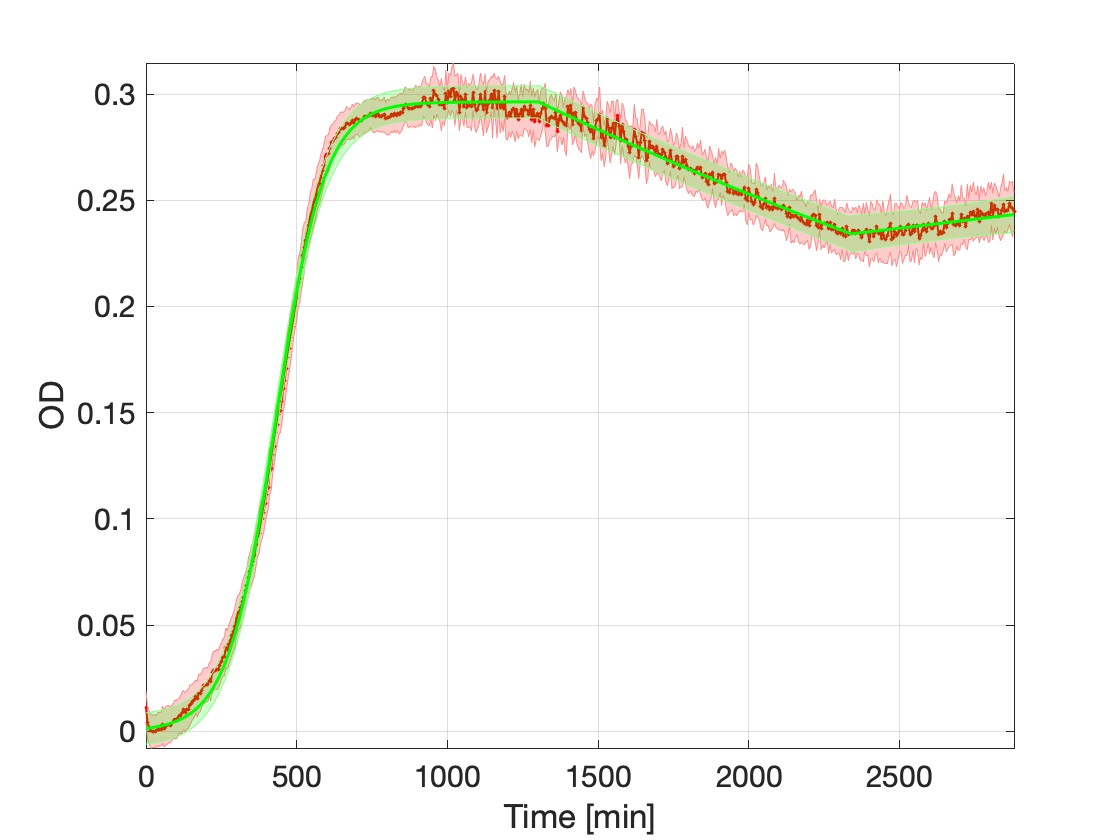
\includegraphics[width=0.6\textwidth]{ex1}
\end{center}

Finally the output is stored
\begin{lstlisting}[frame=single,numbers=left,style=Matlab-Pyglike]
parameters.p{i}(4) = param.mu;
parameters.s{i}(4) = fittedparametersStd(1);
\end{lstlisting}
and saved
\begin{lstlisting}[frame=single,numbers=left,style=Matlab-Pyglike]
DataEXP12= Data; %CHANGE name
experimentEXP12= experiment; %CHANGE name
parametersFitEXP12= parametersFit; %CHANGE name

save('dataRebecca/DataEXP12.mat','DataEXP12') %%CHANGE Data.mat
save('dataRebecca/experimentEXP12.mat','experimentEXP12') %%CHANGE experiment.mat
save('dataRebecca/parametersFitEXP12.mat','parametersFitEXP12') %%CHANGE parametersFit.mat
\end{lstlisting}
Remember to give different names not to overwrite the files.
The last part of the code, just print the results after storing them in a structure
\begin{lstlisting}[frame=single,numbers=left,style=Matlab-Pyglike]
%load all the datasets to plot together
load('dataRebecca/DataEXP1.mat','DataEXP1') %%CHANGE Data.mat
load('dataRebecca/parametersFitEXP1.mat','parametersFitEXP1')  %%CHANGE parametersFit.mat
DataF.p{1} = DataEXP1;
parametersF.p{1} = parametersFitEXP1.p{1};
parametersF.s{1} = parametersFitEXP1.s{1};

load('dataRebecca/DataEXP2.mat','DataEXP2') %%CHANGE bkg.mat
load('dataRebecca/parametersFitEXP2.mat','parametersFitEXP2')  %%CHANGE parametersFit.mat
DataF.p{2} = DataEXP2;
parametersF.p{2} = parametersFitEXP2.p{1};
parametersF.s{2} = parametersFitEXP2.s{1};
\end{lstlisting}

The final result from the fit can be saved in an excel file if a name is provided. To summarise: the best average fit values for the parameters are stored into the vector parametersFit.p and the standard deviation into parametersFit.s following the order of the vector parameters0 [1 klag,2 tlag,3 q,4 mu,5 tswitch,6 kswitch,7 --,8 t--,9 k--,10 tdeath,11 kdeath,12 m, 13 x0, 14 k, 15 k2, 16 k3]. Time are in cycles and not seconds here. DataF.p{i}.XXX contains all the datapoints and std.


\end{document}